\section{}
在\textbf{方向和距离回归}阶段,我们使用一个简单的神经网络(如全连接网络)作为回归模型,输入为图表示学习得到的全局向量 \( H_{\text{global}} \)。模型包含两个输出层:一个用于预测鸟类的方向(上、下、左、右),另一个用于预测鸟类与画面中心的距离。通过结合方向损失(交叉熵损失)和距离损失(均方误差损失),模型在训练阶段学习从全局向量到鸟类方位的映射关系。在监控阶段,即使当前画面中没有鸟,模型也能根据输入的全局向量实时预测鸟类可能出现的方向和距离,并指导监控摄像头转动到对应的方向,以提高监控效率。

\begin{figure}[h!]
\centering %图片居中
\subfloat[方向和距离回归]{
	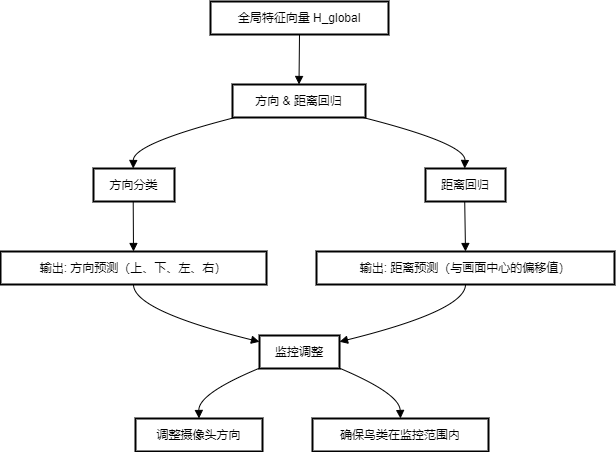
\includegraphics[width=0.9\textwidth]{figures/方向和距离回归.drawio.png}
}
\end{figure}

\paragraph{}
说明:
方向和距离回归:基于全局特征预测鸟类的位置方向(分类)和距离(回归)。
监控调整:根据预测结果实时调整摄像头,保持鸟类在画面中心。